% !TeX root = RJwrapper.tex
\title{\pkg{genpathmox}: An R Package to Tackle Numerous Categorical Variables and Heterogeneity in Partial Least Squares Structural Equation Modeling}
\author{by Giuseppe Lamberti}

\maketitle

\abstract{Partial least squares structural equation modeling (PLS-SEM), combined with the analysis of the effects of categorical variables after estimating the model, is a well-established statistical approach to the study of complex relationships between variables. However,  the statistical methods and software packages available are limited when we are interested in  assessing the effects of several categorical variables and shaping  different groups following different models. Following the framework established by \citet{Lamberti16}, we have developed the  \CRANpkg{genpathmox} \emph{R} package for handling a large number of categorical variables when faced with heterogeneity in PLS-SEM. The package has functions for various aspects of the analysis of heterogeneity in PLS-SEM models, including estimation, visualization, and hypothesis testing. In this paper, we describe the implementation of \pkg{genpathmox} in detail and demonstrate its usefulness by analyzing employee satisfaction data.}

\section{Introduction}

Partial least squares structural equation modeling (PLS-SEM; \citealp{Wold85}) is a method for estimating causal relationships between observed variables and hypothesized latent variables \citep{Evermann21}. PLS-SEM was developed initially as an alternative to the classical covariance based-structural equation modeling (CB-SEM) that estimates latent variables (LVs) as common factors that explain co-variation between the associated indicators \citep{Hair17b}. However, in the last fifteen years it has become a reference for estimating causal models, in particular in marketing and management research \citep{Beker22, Sarstedt22a, Sarstedt22b, Hair21, henseler21, Evermann21}.

Concurrent with the affirmation of the PLS-SEM approach for estimating causal models, there has been a corresponding surge in research addressing the issue of heterogeneity in parameter estimation.This arises when the existence of different models is assumed for data characterized by differences in the coefficients that explain causal relationships between LVs. In this scenario, a single model could provide a biased view of those causal relationships.  The literature describes several approaches to tackling heterogeneity that can be classified in terms of observed heterogeneity, and non-observed heterogeneity (for a detailed review of the PLS-SEM analysis in the presence of heterogeneity, see \citealp{Klesel22})

Observed heterogeneity is based on the hypothesis that the underlying relationship between latent variables vary by certain categorical variables (CVs), for example sociodemographic factors such as gender, education, or social status, such that the data can be separated into groups and a different model can be fit to each group. The presence of observed heterogeneity is then verified by testing whether the coefficients of the estimated models are significantly different between groups \citep{Hair17}. Belonging to this category are the classical PLS multigroup tests, including the parametric \citep{Keil00}, permutation \citep{Chin10}, and Henseler \citep{Henseler09} tests, as well as the more recent approach proposed by \citet{Klesel19}. As for non-observed heterogeneity, this is present when differences are inherent to the data. In this scenario, a different approach is required, and different models are typically identified following a latent class analysis \citep{Sarstedt22c} or clustering \citep{Vinzi08} approach.

Methodological advances and the increase in applications have led to the development of numerous  \emph{R} packages, starting with  \CRANpkg{plspm} \citep{plspm}, subsequently followed by  \CRANpkg{cSEM} \citep{csem} and  \CRANpkg{SEMinR} \citep{seminr}, both of which incorporate recent developments in the PLS approach, including improved estimation (consistent PLS  (PLSc) \citealp{Dijkstra15}), improved validation criteria  (the PLSpredict approach to prediction \citealp{Shmueli16,Shmueli19}),  new reliability measures \citep{Dijkstra15, Hair19}, and also \CRANpkg{matrixpls} \citep{matpls}, particularly used for simulation studies. Concerning heterogeneity,  the \pkg{cSEM} package allows multigroup analysis with several embedded tests. 
Pathmox analysis \citep{Sanchez06, Lamberti16, Lamberti17}  was proposed as a useful method when observed heterogeneity is assumed, but several potential CVs exist that could define different groups and models. This method explores and identifies, using an iterative algorithm, the most significantly different groups associated with significant differences in models. The algorithm follows a segmentation tree approach, where each node is a PLS-SEM model. Differences are compared and partitions are chosen that define the most significant divergences between coefficients \citep{Lamberti16}.  The algorithm has been further improved, first by including a statistical test capable of identifying, for each split, the model coefficient responsible for the partitions \citep{Lamberti17}, and then by combining the pathmox algorithm with classical multigroup analysis in a new approach called hybrid multigroup analysis  \citep{Lamberti21}. 

In this paper, we describe the \CRANpkg{genpathmox} package \citep{genpathmox} which implements the classical pathmox analysis and the more recently developed hybrid multigroup analysis \citep{Lamberti21}. The package, initially developed in 2014,  has been updated to include recent methodological advances (including PLSc;  \citealp{Dijkstra15}) and has also been modified to work jointly with the  \pkg{cSEM} package to increase analytical flexibility. Below we first review the framework formalized by \citet{Lamberti16}, then provide an overview of the \pkg{genpathmox} package, and finally, we demonstrate the use of the package on real-world analysis of employee satisfaction data and work climate drivers.

\section{Overview of the pathmox methodology}

Pathmox analysis  \citep{Lamberti16, Lamberti17} was introduced to handle observed heterogeneity in PLS-SEM when several CVs are present.  Unlike classical methods for tackling observed heterogeneity in PLS-SEM, instead of testing whether a CV produces a significant difference in model coefficients (i.e., a confirmatory approach),  an exploratory approach is adopted. That is, the aim of pathmox is to identify siginificantly different groups associated with different PLS models, provided they exist. The algorithm applies a binary tree partitioning approach. It first estimates a single global model for the entire dataset to define the root node of the tree, and then explores all possible binary partitions for each CV. Differences in coefficients are statistically evaluated by the $F$-global test  \citep{Lamberti16}. This test provides a global measure of the degree of difference between partitions (i.e., a $p$-value).  Comparisons are then sorted  in descending order based on the $p$-values, and the partition with the smallest $p$-value (i.e. one which suggests the greatest difference from the root model) is then chosen as optimal. 

The degree of difference between models (the split criterion) is determined by applying a test, inspired by  \citet{Chow60} and \citet{Lebart79} which compares differences between the coefficients of two linear regression models. In pathmox, the difference between two PLS-SEM models is determined by comparing structural model coefficients, i.e., by comparing, as in the case of \citet{Chow60} and \citet{Lebart79}, restricted deviance vs. unrestricted deviance, defined, respectively, as the deviance calculated for the whole sample considering a single model valid for all the observations, and the sum of the model deviances estimated for each group of observations.  

From a graphical standpoint, pathmox is not much different from a classical segmentation tree -- as the algorithm produces a tree with a root, intermediate nodes, and terminal nodes -- other than that each node is associated with a PLS model. 

\subsection{The split criterion}

The split criterion used to define the tree partitions is a critical aspect of the pathmox algorithm. Below we describe the $F$-global test, the formulation of the null and alternative hypotheses, and the statistic used to test the null hypothesis (further details are available in \citealp{Lamberti16}).

Consider a simple structural model with one dependent LV, denoted by the Greek letter \textbf{$\eta$}, and explained by a generic set of independent LVs denoted by the matrix  \textbf{X} = $\{\xi_{ip}\}$, where $i = 1, \ldots, n$ refers to the observation, and where $p = 1, \ldots, P$ refers to the LV. Its generalization into a more complex model is straightforward. 

Using the matrix form, the model can be expressed as: 
\begin{equation}
\label{eq1}
\boldsymbol{\eta} = \textbf{X}\boldsymbol{\beta} + \boldsymbol{\varepsilon}
\end{equation}
where $\boldsymbol{\beta}$ is the vector  of the regression coefficients of $\boldsymbol{\eta}$, and where $\boldsymbol{\varepsilon}$ is the disturbance term. Let the data  be partitioned by rows, where the partition is determined by a CV  with  \textit{m} categories (i.e., segments or groups). The number of units in group \textit{g} ($g=1,\ldots, m$) is denoted by $n_g$, and  the total sample size can be expressed as $n=\sum_{g=1}^m n_g$.
The $F$-global test compares model coefficients only by considering binary partitions. This means that the number of comparisons depends on the nature of the CVs. With a dummy (binary) CV, there is just a single comparison.  With a nominal CV, there are $2^{m-1}-1$ comparisons. Finally, with an ordinal CV, there are $m-1$ comparisons.

The logic of  the test is to compare the coefficients of two models, while considering two different scenarios. Under the null hypothesis, we assume that one model is valid for all observations. This implies  that one coefficient for each independent LV is enough to explain the dependent LV.  If we  consider the simplest case of a dummy CV (\textit{m}=2), denoting the two groups as $A$ and $B$, the null and alternative hypotheses can be formulated as:

\begin{align}
\label{eq2}
H_0: \boldsymbol{\beta}_A = \boldsymbol{\beta}_B \\
H_1: \boldsymbol{\beta}_A \ne \boldsymbol{\beta}_B
\end{align}
According  to the null and alternative hypotheses, and following \citet{Lebart79},  we can rearrange Eq. \ref{eq1} as follows:  

\begin{equation}
\label{eq22}
\left[\begin{array}{l}
\boldsymbol{\eta}_A \\
\boldsymbol{\eta}_B 
\end{array}\right] \quad
\left[\begin{array}{l}
\textbf{X}_A \\
\textbf{X}_B 
\end{array}\right] \quad
\left[\begin{array}{l}
\boldsymbol{\beta}
\end{array}\right]  \quad +
\left[\begin{array}{l}
\boldsymbol{\varepsilon}_A \\
\boldsymbol{\varepsilon}_B 
\end{array}\right] 
\end{equation}

\begin{equation}
\label{eq23}
\left[\begin{array}{l}
\boldsymbol{\eta}_A \\
\boldsymbol{\eta}_B 
\end{array}\right] \quad
\left[\begin{array}{cc}
\textbf{X}_A \quad0\\
0 \quad\textbf{X}_B 
\end{array}\right] \quad
\left[\begin{array}{l}
\boldsymbol{\beta}_A \\
\boldsymbol{\beta}_B
\end{array}\right]  \quad +
\left[\begin{array}{l}
\boldsymbol{\varepsilon}_A \\
\boldsymbol{\varepsilon}_B 
\end{array}\right] 
\end{equation}

We calculate the deviance (the sum of squared residuals, SSR) for both models: $SSR_{H0}$ under the null hypothesis and $SSR_{H1}$ under the alternative. Finally, we test the null hypothesis using the following statistic:

\begin{equation}
\label{F_global}
F  = \frac{\left(SSR_{H_0}-SSR_{H_1}\right) \Bigg/p}{SSR_{H_1}\Bigg/n-2p}   
\end{equation}
which follows an $F$ distribution with $p$ and $\left(n - 2p\right)$ degrees of freedom, where $p$ is the number of explanatory LVs, and where $n = n_A + n_B$ is the total number of observations.

\subsection{Improving tree partition interpretation: the $F$-coefficient test}

The $F$-coefficient test was an important improvement in the algorithm introduced in \citet{Lamberti17}. The $F$-global test used in pathmox as a split criterion is a global criterion that establishes whether or not the CV reflects a significant difference. However, it does not provide information as to which coefficients are responsible for that difference.  The $F$-coefficient test complements the split criterion in pathmox by providing information about which coefficients may be responsible for the significant difference.

Rearranging  the model formulated by Eq. \ref{eq1}, we consider the particular case of one dependent LV denoted $\eta$, and two predictor LVs denoted $\xi_1$ and $\xi_2$: 

\begin{equation}
\label{eq4}
\boldsymbol{\eta} = \boldsymbol{\xi}_1\beta_1 + \boldsymbol{\xi}_2\beta_2 + \boldsymbol{\varepsilon}
\end{equation}

Let us assume that a significant difference exists between the models estimated for the two groups,  $A$ and $B$,  as defined by a generic dummy variable. Applying the $F$-global test \citep{Lamberti16} we cannot determine whether the difference between the two models depends on  $\xi_1$ or $\xi_2$, or depends on both. However the null hypotheses for $\beta_1$ and $\beta_2$, and the corresponding alternative hypotheses, can be reformulated to determine whether the coefficients estimated for the predictors are significantly different, as follows:\footnote{Note that the alternative hypothesis is the same for both  $\xi_1$ and $\xi_2$.} 
\begin{align}
\label{eq5}
H_0: &\beta_{iA} =\beta_{iB}  \quad  \text{with i }= 1, 2\\
H_1: &\boldsymbol{\beta}_A \ne \boldsymbol{\beta}_B
\end{align}
According to the null and alternative hypotheses, and following \citet{Lebart79},  we can rearrange Eqs. \ref{eq22} and \ref{eq23}  as:  

\begin{equation}
\label{nul2}
\left[\begin{array}{l}
\boldsymbol{\eta}_A \\
\boldsymbol{\eta}_B 
\end{array}\right] \quad
\left[\begin{array}{ccc}
\boldsymbol{\xi}_{1A}\quad 0 \quad0\\
0 \quad\boldsymbol{\xi}_{2A} \quad0\\
\boldsymbol{\xi}_{1B} \quad0 \quad0\\
0 \quad0 \quad\boldsymbol{\xi}_{2B}\\
\end{array}\right] \quad
\left[\begin{array}{l}
\beta_1 \\
\beta_{2A} \\
\beta_{2A} \\
\end{array}\right]  \quad +
\left[\begin{array}{l}
\boldsymbol{\varepsilon}_A \\
\boldsymbol{\varepsilon}_B 
\end{array}\right] 
\end{equation}

\begin{equation}
\label{nul22}
\left[\begin{array}{l}
\boldsymbol{\eta}_A \\
\boldsymbol{\eta}_B 
\end{array}\right] \quad
\left[\begin{array}{ccc}
\boldsymbol{\xi}_{1A}\quad 0 \quad0\\
0 \quad\boldsymbol{\xi}_{2A} \quad0\\
0 \quad0 \quad\boldsymbol{\xi}_{1B}\\
0 \quad\boldsymbol{\xi}_{2B} \quad0\\
\end{array}\right] \quad
\left[\begin{array}{l}
\beta_{1A} \\
\beta_{1B} \\
\beta_2 \\
\end{array}\right]  \quad +
\left[\begin{array}{l}
\boldsymbol{\varepsilon}_A \\
\boldsymbol{\varepsilon}_B 
\end{array}\right] 
\end{equation}

\begin{equation}
\label{al2}
\left[\begin{array}{l}
\boldsymbol{\eta}_A \\
\boldsymbol{\eta}_B 
\end{array}\right] \quad
\left[\begin{array}{ccc}
\boldsymbol{\xi}_{1A}\quad 0 \quad0 \quad0\\
0 \quad\boldsymbol{\xi}_{2A}\quad0 \quad0\\
0 \quad0 \quad\boldsymbol{\xi}_{1B} \quad0\\
0 \quad0 \quad0 \quad \boldsymbol{\xi}_{2B}\\
\end{array}\right] \quad
\left[\begin{array}{l}
\beta_{1A} \\
\beta_{1B} \\
\beta_{2A} \\
\beta_{2B} \\
\end{array}\right]  \quad +
\left[\begin{array}{l}
\boldsymbol{\varepsilon}_A \\
\boldsymbol{\varepsilon}_B 
\end{array}\right] 
\end{equation}

We calculate again the deviance for both models ($SSR_{H0}$ and $SSR_{H1}$) and test the null hypothesis using the following statistic: 

\begin{equation}
\label{F_coefl}
F_i  = \frac{\left(SSR_{H_{0_{\beta_i}}}-SSR_{H_1}\right) \Bigg/1}{SSR_{H_1}\Bigg/2\left(n-\sum p\right)}  \; \text{with i=1,2}
\end{equation}
which follows an $F$ distribution with $1$ and $2\left(n - \sum p\right)$ degrees of freedom, and where $p$ is the number of explanatory LVs, and  $n = n_A + n_B$ is the total number of observations.

Note that both the $F$-global and the $F$-coefficient are implemented in the \pkg{genpathmox} package.

\subsection{Stop criteria}

Since pathmox is an iterative algorithm, its convergence depends on the specific stop criteria adopted by the user.  Three criteria (all implemented in the \pkg{genpathmox} package) are proposed in \citet{Lamberti16}:

\begin{enumerate}
\item A more significant partition is not found. This means that the null hypothesis is not rejected in any of the candidate partitions, and as the obtained models are similar to each other, it makes no sense to continue splitting the data. This condition is also strictly related to the significance threshold of the $p$-value chosen by the user, usually set to 0.05 (a typical $p$-value threshold in PLS-SEM applications).

\item Maximum tree depth is achieved. This is related to the number of terminal nodes required by the user, a choice based on the complexity of the model and the number of CVs used. Generally speaking, trees of 2-3 levels (with a maximum of 4-8 associated terminal nodes) are preferred.\footnote{A greater tree depth results in a higher number of terminal nodes, with the direct consequence of having to make more comparisons between model coefficients, and with results that may not always be easy to interpret.}

\item A node has too few observations to be partitioned. PLS-SEM works well with a relatively small number of observations, but it is recommended to fix a threshold of a relatively large number of observations to ensure that nodes are representative. For exploratory purposes, the recommended number of observations in each node is between 50 and 100.  

\end{enumerate}

\subsection{Pathmox to reduce the number of comparisons before running multigroup analysis: hybrid multigroup analysis}

A criticism of the multigroup approach is that differences between coefficients could be difficult to interpret when the number of comparisons is high.  This could happen when we have to simultaneously analyze more than one CV, or when the CV has more than 3 or 4 levels. 

The pathmox algorithm does not perform an a posteriori statistical comparison of the coefficients of the models associated with the terminal nodes, nor does it establish the invariance between groups that is an important aspect of comparing PLS-SEM models \citep{Henseler16}.\footnote{Invariance ensures that a dissimilar group-specific model estimate does not depend on diverse LV meaning across groups. A specific procedure to verify measurement invariance in the PLS-PM framework – proposed by \citet{Henseler16} – is measurement invariance of composite models (MICOM), consisting of three hierarchical steps: (1) configural invariance, which ensures the same LV specifications when LVs are equally parameterized and estimated across groups, (2) compositional invariance, which ensures that LV scores reflect the same construct across groups, and (3) equality of latent variables, which means that values and variances ensure that data can be pooled across groups. If all three steps are confirmed, full measurement invariance is established, while if only the first two steps are confirmed partial measurement invariance is established. Step one and two are necessary condition for performing multigroup analysis. A practical guideline on applying MICOM  is provided by \citep{Hair17}, while \citet{Henseler16} provide more details on methodological aspects.} However, pathmox can be used just to reduce the number of groups to compare before running a classical multigroup analysis. Instead of using the original CV, the multigroup comparison uses a new intersection CV defined by the CV groups resulting from the tree partitions. This is called the hybrid segmentation variable \citep{Lamberti21}, which is used for the hybrid multigroup analysis.  

The hybrid multigroup analysis consists of sequential steps as follows:

\begin{enumerate}
\item Use pathmox to identify the most significantly different groups
\item Use multigroup analysis to compare the groups:
\begin{enumerate}
\item Test the invariance of the constructs among groups using the MICOM procedure \citep{Henseler16}
\item Test the statistical differences between models using a criterion proposed by the literature \citep{Klesel22}.
\end{enumerate}
\end{enumerate}

Note that the \pkg{genpathmox} package does not include any function to automatically  run the hybrid multigroup analysis. Rather, this analysis is done, as will be shown below, by combining the \pkg{genpathmox} and \pkg{cSEM} (using the functions  \code{testMICOM()} to test invariance, and  \code{testMGD()} to compare coefficients). 

\subsection{Pathmox advantages and limitations}

A first advantage of pathmox is that, given a set of CVs, it yields the most significantly different groups associated with the most significantly different models. The algorithm reduces the number of groups to be compared and analyzed, with the direct consequence that the user merely has to interpret the differences. A second advantage is that it ranks CVs by their importance in the split process (as in other classical tree partitioning procedures). This is important because an analysis of differences in PLS-SEM with more CVs involves not only comparing groups, but also establishing the most significant sources of heterogeneity in defining differences.

The main limitation of pathmox is related to the split criteria. The fact that the algorithm realizes an exhaustive search over unadjusted $p$-values to determine the best partition could potentially produce biased results \citep{loh97}. A possible solution would be to apply a Bonferroni correction for multiple comparisons, but  this is not yet available in the current version of the package. The $F$-global and the $F$-coefficients are parametric tests based on a classical parametric statistic: the $F$-statistic. This supposes the normality assumption of the perturbation terms with equal variance in all dependent constructs, even though the assumptions are rarely met in practice. Nevertheless, the sensitivity of the $F$-statistic is guaranteed by a larger sample size, lower levels of random perturbations, and clearer differences in the segments, as shown by the simulations performed by \citet{Lamberti16, Lamberti17}.
Another important limitation is that pathmox focuses only on the problem of detecting the path coefficients that are responsible for differences between PLS-SEM models, by adapting the measurement model to each segment. This leads to the problem of invariance, which greatly increases in importance when we analyze data with potential sources of heterogeneity by fitting one model to each segment. In this situation, it could become difficult to guarantee that each construct in each segment is measuring the same latent construct.

Finally, it is important to remark that the $F$-tests are determined by the sum of the squares of the residuals of the structural model in parent and children nodes and using the composite scores. Indeed, in the case of the common factor, the composites scores can just be used as common factor proxies since they are contaminated by measurement random error. Hence, the $F$-test ranking of the CVs may not be optimum when there is a small number of indicators per latent variable. Researchers who intend to apply pathmox when common factors are present in the model should take this limitation into account in performing the analysis; alternatively they should use the classical PLS algorithm modifying the options of the \pkg{genpathmox} functions accordingly.

\section{The \emph{genpathmox} package}

\subsection{Overview}

The \pkg{genpathmox} package is based on one main function called  \code{pls.pathmox()}, which implements the pathmox algorithm and provides results for analysis. Four additional functions are a  \code{summary()} function, and three plot functions (\code{plot()},  \code{bar\_impvar()},  \code{bar\_terminal()})  that help the user to interpret results. In practice, users should first apply the main function  \code{pls.pathmox()} to generate a  "\code{plstree}" object.  The components of this object include tree partition results, fitted coefficients of the PLS models for each terminal node, and other results to be used for the analysis. The  "\code{plstree}" object plays an instrumental role, as it is a necessary input for the other functions in the package. This design is convenient, as details of data, PLS model, and tree split rules need only be specified once in  \code{pls.pathmox()}, and are passed to other functions.

The  \code{summary()} function provides a complete output of all results,  \code{plot()} provides the segmentation tree plot,  \code{bar\_impvar()} provides a bar plot of the ranking by importance of the CVs that participate in the split process, and   \code{bar\_terminal()}  produces a bar plot of the coefficients of the PLS terminal nodes of the tree, enabling intuitive analysis of the differences between them.

The \pkg{genpathmox} package has been designed to interact with the \pkg{cSEM} package \citep{csem}, one of the latest and  most complete packages for PLS-SEM analysis. This package can be used to analyze each model associated with the terminal nodes identified by pathmox and to run the hybrid multigroup analysis. To that end, the  "\code{plstree}" object also contains a list of datasets called \code{.hybrid}, corresponding to lists of datasets of observations belonging in the tree terminal nodes. 

Using the \code{.hybrid} list combined with the \pkg{cSEM::csem()}, each terminal node can be easily and completely analyzed  in terms of model validation, coefficient estimation, and inference. The resulting object generated by \code{csem()} can then be passed to  \code{testMICOM()} to verify the invariance of the model constructs for the terminal nodes, and to  \code{testMGD()} to compare the coefficients. The hybrid multigroup approach \citep{Lamberti21} can then be implemented. Further details on how to use the \pkg{cSEM} package are available in \citet{csem}. 

Figure ~\ref{figure:flow} illustrates how to use the \pkg{genpathmox} package. On the left, the grey block contains the input elements, i.e., the data, the model, and the tree rules. Calling up \code{pls.pathmox()} generates the  "\code{plstree}" object, as shown in the central orange block, which yields estimation and visualization results, as shown in the two orange blocks on the right. Finally,  \code{plstree\$hybrid} is used as the input parameter of the \pkg{cSEM} package, yielding full results for the terminal nodes and the multigroup analysis, as shown in the blue  blocks. 

\begin{figure}[htbp]
  \centering
  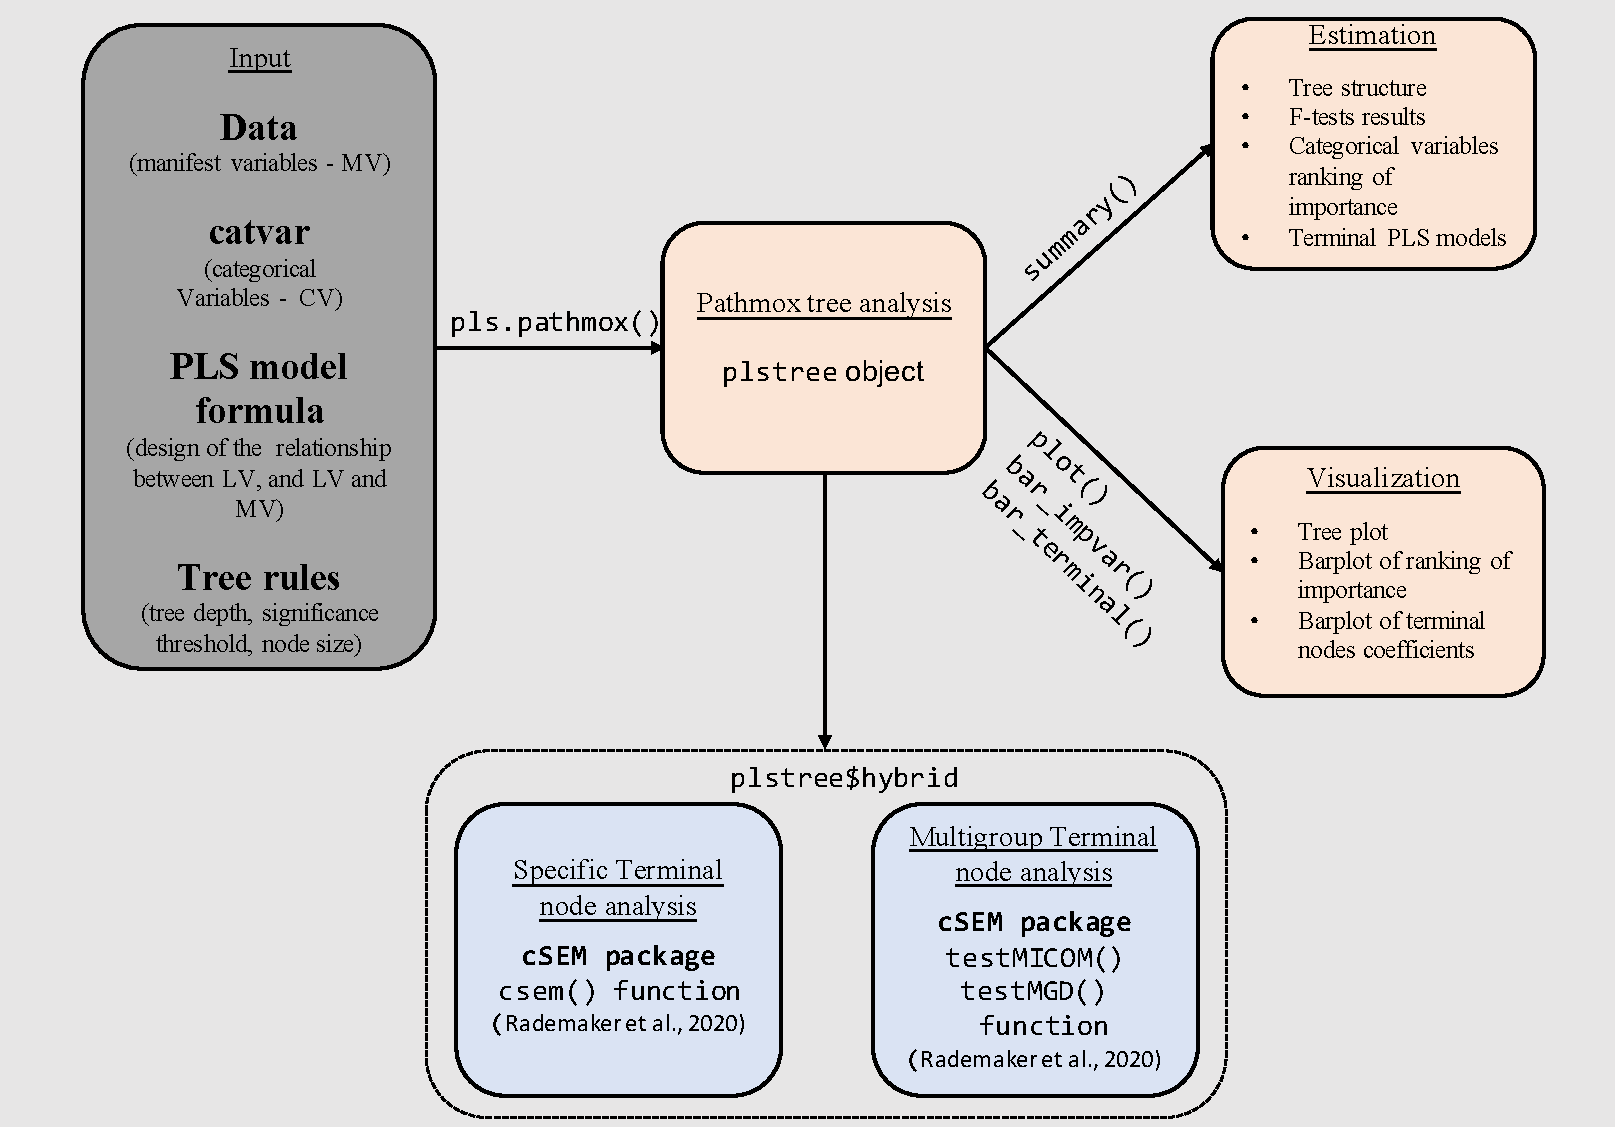
\includegraphics[height=8cm]{Fig1_flow}
  \caption{Illustration of \pkg{genpathmox} package functions}
  \label{figure:flow}
\end{figure}


\subsection{Implementation of main functions}

\subsection{Estimation function: \code{pls.pathmox}}

To apply the \code{pls.pathmox} function, users need to specify at least three arguments: 

\begin{enumerate}
\item  \code{.model}. A formula specifying the model described using syntax inspired by the lavaan package \citep{lavaan}. Structural and measurement models are defined by enclosure between double quotes. The directional link between constructs is defined using the ("$\sim$") operator. The dependent LV is on the left-hand side of the operator, and the explanatory LVs, separated by the ("+") operator, are on the right-hand side. As for the outer model, LVs are defined by listing the corresponding indicators after the operator ("$=\sim$") if the LV is modelled as a common factor, or the operator("$<\sim$") if the LV is modelled as a composite. On the left-hand side of the operator is the LV, and on the right-hand side are the indicators separated by the ("+") operator. Please note that variable labels cannot contain (".") (for details of the meaning of modes A and B, see \citealp{Hair16}).
\item  \code{.data}. A matrix or data frame containing the indicators. 
\item  \code{.catvar}. A single factor or set of factors organized as a data frame containing the CVs used as sources of heterogeneity.
\end{enumerate}

Other input parameters have default values.  Table ~\ref{par_imp} reports the meaning of each parameter and the admissible and default values. 

\begin{table}[htbp]
\begin{tabular}{p{2cm}p{4.25cm}p{4.25cm}p{1.4cm}}
\toprule
{Parameter} & {Purpose} & {Possible values} & {Default values}\\
\midrule
 \code{.scheme}& inner weighting scheme &  "\code{centroid}",  "\code{factorial}", or "\code{path}"&  "\code{path}"\\ 
  \code{.consistent}& consistent PLS estimation \citep{Dijkstra15} is used instead of classical approach \citep{Wold85}&  \code{TRUE} or  \code{FALSE}& \code{TRUE}\\ 

 \code{.alpha}& minimum threshold significance & values belonging the interval $[0,1]$& 0.05\\
 \code{.deep}& maximum tree depth & an integer $\geq$ 1& 2\\
 \code{.size}& minimum proportion of total sample admissible for a node size&value belonging the interval $[0,1]$ & 0.10\\
 \code{.candidate size}& minimum admissible size for a candidate node&an integer $\geq$ 0 &  50\\
 \code{.tree}& logic parameter to show the tree plot&  \code{TRUE} or  \code{FALSE}&  \code{TRUE}\\
\bottomrule
\end{tabular}
\caption{Input parameters with default values \label{par_imp}}
\end{table}

Once the split process is complete, results are saved in the object of class "\code{plstree}" , which contains all the results necessary to interpret the pathmox analysis (see Table ~\ref{output})

\begin{table}[htbp]
\begin{tabular}{p{2.2cm}p{10.6cm}}
\toprule
{Results} & {Use}\\
\midrule
 \code{MOX}& provides information on the tree structure: node type (intermediate or terminal), node size, binary split\\ 
 \code{terminal\_paths}& allows visualization of path coefficients and $R^2$ for each terminal node\\
 \code{var\_imp}& provides a ranking of the CVs used in the split process\\
 \code{Fg.r}& identifies which CV is responsible for the partition\\
 \code{Fc.r }& identifies the path coefficient responsible for the partition\\
 \code{hybrid}& subsets of data associated with each terminal node\\
\bottomrule
\end{tabular}
\caption{"\code{plstree}" results \label{output}}
\end{table}


\subsection{Visualization functions: \code{plot}, \code{bar\_impvar} and  \code{bar\_terminal}}

Three types of plots are possible in the  \textbf{genpathmox}  package: a pathmox treeplot, a barplot which displays the ranking of the CVs, and a barplot of the PLS-SEM coefficients of the terminal nodes. The tree plot is obtained by applying the \code{plot()} function, which returns a tree structure with root, intermediate, and terminal nodes. For each partition, the $F$-global test $p$-value is reported with the associated CV, and the number of observations associated with each node. The plot is implemented using functions from the \pkg{diagram} package \citep{diagram}. The plot of the CV ranking is obtained using the  \code{bar\_impvar()} function. This function uses the  \code{barplot()} function to visualize the importance of the CVs. The importance of  each CV is based on the $F$-statistic of the $F$-global test calculated for each CV in each tree node. Finally, the plot of the coefficients of the PLS-SEM model for each terminal node is obtained using the  \code{bar\_terminal()} function, also based on the  \code{barplot()} function, which allows a more intuitive comparison of the coefficients of the terminal nodes. 

The user can choose between two bar plot visualizations: (1) a plot of all the coefficients of the same model in the same plot, which is useful for comparing the terminal nodes models, and (2) a plot of the same coefficients for all terminal nodes in the same plot (lines correspond to the coefficients and bars report the coefficient effects), useful for a more direct comparison of a specific coefficient between models. In the former, the bar plot depicted for each model also plots the associated $R^2$. Visualization options are selected by modifying the  \code{.bycoef} parameter. By default, this is set to  \code{FALSE}, meaning that the function implements the first option. We also need to specify for which dependent LV we want to visualize the predictor effect by fixing the parameter  \code{.LV = }" ", which we do by indicating the dependent LV between quotation marks.

\section{ Application: analysis of employee satisfaction in terms of work climate drivers}

The use of the \pkg{genpathmox} package is illustrated using real-world data on employee satisfaction in an international Spanish bank. In the financial sector, the impact of work climate on the relationship between strategic human resource management and organizational performance is crucial, in particular among younger employees \citep{Kollmann20}. Another issue of relevance is that different groups of employees may respond in different ways to specific human resource management practices \citep{Lamberti20}.
The data of a sample of younger employees ($\leq$30 years) of the Spanish bank contain measures regarding satisfaction (SAT), loyalty (LOY), and five work climate constructs: empowerment (EMP), company reputation (REP), leadership (LEAD), pay (PAY), and work conditions (WC). Our model relates the five work climate constructs with SAT, and SAT with LOY. Each construct is represented by a specific set of indicators. Information is also available on gender (female 53.36\%), job level (intermediate, 52.01\%), and seniority (length of service < 5 years, 66.81\%).  

Full details of indicators and LVs are available in the  \pkg{genpathmox} manual, and details of the theoretical framework are provided in \citet{Lamberti20}.

Our objectives were: (1) to identify defining characteristics of different groups of employees, and (2) to analyze differences in the models for those groups.

 \subsection{Estimation}
 
We used the  \code{pls.pathmx()} function to partition the tree according to the CVs. We specified in order the parameter of the function \code{pls.pathmx()}:  the model (\code{.model}), (2) the data (\code{.data}), and  (3) the CVs (\code{.catvar}).  The other parameters  were left at the default values. We defined a structural model relating the five work climate constructs (EMP, REP,  LEAD, PAY, WC) with SAT, and SAT with LOY, and we then related each construct to its own set of indicators (measurement model). 

Note that, in this example, LVs are estimated as common factors. Indeed, by fixing the parameter \code{ .consisten = TRUE}, consistent PLS estimation \citep{Dijkstra15} will only have an effect on the final estimation of the path coefficients of the models of terminal nodes as identified by pathmox. Composite scores will be used to calculate the $F$-statistic, and to identify potential sources of heterogeneity.
 


\begin{example}
# load genpathmox package
library(genpathmox)

# load data
data(climate)

# define del model  
climate_model  =  "
	# structural model 
	SAT ~ EMP + REP + PAY + WC + LEAD
	LOY ~   SAT
	# measurement model
	EMP =~ Empo1 + Empo2 + Empo3 + Empo4 + Empo5 
	REP  =~ Imag1 + Imag2 + Imag3     
	PAY  =~ Pay1+ Pay2 + Pay3 + Pay4
	WC =~ Work1 + Work2 + Work3
	LEAD =~ Lead1 + Lead2 + Lead3 + Lead4 + Lead5
	SAT =~ Sat1 + Sat2 + Sat3 + Sat4 + Sat5 + Sat6
	LOY =~ Loy1 + Loy2 + Loy3
	"
# define the set of categorical variables
climate_catvar = climate[,1:3]

# run the pls.pathmox() function
climate.pathmox = pls.pathmox(
	.model = climate_model,
	.data = climate,
	.catvar = climate_catvar)

PLS-SEM PATHMOX ANALYSIS 

---------------------------------------------
Info parameters algorithm 
  parameters algorithm value
1    threshold signif.  0.05
2   node size limit(\%) 0.10
3     tree depth level  2.00

---------------------------------------------
Info segmentation variables 
          nlevels ordered treatment
Level           3    TRUE   ordinal
Seniority       2    TRUE    binary
Gender          2   FALSE    binary

\end{example}

As shown above, the default output of the  \code{pls.pathmx()} function is a  table containing the stop criteria and the  list of CVs used in the split partitions. Below we use the  \code{summary()} function to interpret the results.

 \begin{example}
summary(climate.pathmox)

PLS-SEM PATHMOX ANALYSIS 

---------------------------------------------
Info parameters algorithm: 
  parameters algorithm value
1     threshold signif  0.05
2   node size limit(%)  0.10
3     tree depth level  2.00
---------------------------------------------
Info tree: 
        parameters tree value
1             deep tree     2
2 number terminal nodes     3
---------------------------------------------
Info nodes: 
  node parent depth  type terminal size      % variable   category
1    1      0     0  root       no  669 100.00     <NA>       <NA>
2    2      1     1  node       no  476  71.15    Level low/medium
3    3      1     1 least      yes  193  28.85    Level       high
4    4      2     2 least      yes  258  38.57   Gender     Female
5    5      2     2 least      yes  218  32.59   Gender       Male
---------------------------------------------
Info splits: 

Variable: 
  node variable     g1.mod g2.mod
1    1    Level low/medium   high
2    2   Gender     Female   Male





Info F-global test results (global differences): 
     node F value Pr(>F)    
[1,]    1  6.9711 <2e-16 ***
[2,]    2  3.0647 0.0021 ** 
---
Signif. codes:  0 ‘***’ 0.001 ‘**’ 0.01 ‘*’ 0.05 ‘.’ 0.1 ‘ ’ 1

Info F-coefficient test results (coefficient  differences) : 

Node 1 :
            F value Pr(>F)  
EMP -> SAT   2.5902 0.1078  
REP -> SAT   0.4056 0.5243  
PAY -> SAT   3.6390 0.0567 .
WC -> SAT    0.7342 0.3917  
LEAD -> SAT  4.1333 0.0422 *
SAT -> LOY   0.1044 0.7467  
---
Signif. codes:  0 ‘***’ 0.001 ‘**’ 0.01 ‘*’ 0.05 ‘.’ 0.1 ‘ ’ 1

Node 2 :
            F value Pr(>F)    
EMP -> SAT   0.0229 0.8797    
REP -> SAT   0.6333 0.4263    
PAY -> SAT   0.1874 0.6652    
WC -> SAT    0.9907 0.3198    
LEAD -> SAT  2.5447 0.1110    
SAT -> LOY  17.9754 <2e-16 ***
---
Signif. codes:  0 ‘***’ 0.001 ‘**’ 0.01 ‘*’ 0.05 ‘.’ 0.1 ‘ ’ 1
---------------------------------------------
Info variable importance ranking: 
   variable   ranking
2     Level 0.3949974
3 Seniority 0.3101112
1    Gender 0.2948914
---------------------------------------------
Info terminal nodes PLS-SEM models (path coeff. & R^2): 
          node 3 node 4 node 5
EMP->SAT  0.1233 0.2051 0.2725
REP->SAT  0.3037 0.1548 0.1238
PAY->SAT  0.0798 0.2863 0.1290
WC->SAT   0.4222 0.1333 0.3768
LEAD->SAT 0.2283 0.3283 0.1545
SAT->LOY  0.6934 0.7582 0.8806
R^2 SAT   0.6831 0.6863 0.6597
R^2 LOY   0.4808 0.5749 0.7754
\end{example}

We can interpret the \code{summary()} results as follows:

\begin{enumerate}
\item Pathmox indicates that different groups of employees exist that define SAT and LOY differently.
\item The variables that stratify the different groups of employees are, in order: job level ($F$-statistic = 6.971, $p$-value <0.001), gender ($F$-statistic = 3.065, $p$-value = 0.002). That this, the analysis suggests that employees are  first partitioned into low/intermediate level employees versus high level employees, and low/intermediate level employees are then partitioned according to  gender. 
\item The coefficients responsible of the first split  are  LEAD-->SAT   ($F$-statistic = 4.133, $p$-value = 0.042),  and for the second split, SAT-->LOY  ($F$-statistic = 17.975, $p$-value < 0.001).
\item Pathmox ultimately identifies three groups associated to the terminal tree nodes:  high level employees (node 3), female low level employees (node 4), and male low level employees (node 5).
\item The CV ranking reveals that the most important differentiating characteristic for SAT and LOY is job level, followed by seniority, and finally gender.
\item  In terms of work climate drivers defining SAT, the model comparisons indicate that: 
\begin{enumerate}
\item  High level employees (node 3) are least motivated by EMP ($\beta = 0.123$) and most motivated by WC $\beta = 0.422$) and REP ($\beta = 0.303$). 
\item Female low level employees (node 4) are most motivated by LEAD ($\beta = 0.328$), PAY ($\beta = 0.286$), and EMP ($\beta = 0.205$). 
\item  Male low level employees (node 5) are most motivated by WC ($\beta = 0.377$) and least motivated by REP ($\beta = 0.124$), and also are the employees with the highest $R^2$ for  LOY (0.775).
\end{enumerate}
\end{enumerate}


\subsection{Visualization}

The  \code{summary()} output can be complemented by plots. First,  the  \code{plot()} function, as applied to the object of class "\code{plstree}", produces the tree plot. The \code{bar\_impvar()} and  \code{bar\_terminal()} functions allow graphical visualization of the ranking of CVs and a  comparison of the coefficients (default value  \code{bycoef = FALSE}, and  \code{LV =}  "\code{SAT}" to show the predictors of SAT most relevant for the analysis of work climate drivers). The three plots are shown in Figure \ref{vis}. 

 \begin{example}
# treeplot
plot(climate.pathmox)
# ranking of CVs
bar_impvar(climate.pathmox)
# coefficients comparison
bar_terminal(climate.pathmox, .LV = "SAT")
 \end{example}

\vspace{0.4cm}
\begin{figure*}[t!]
$\begin{array}{rl}
    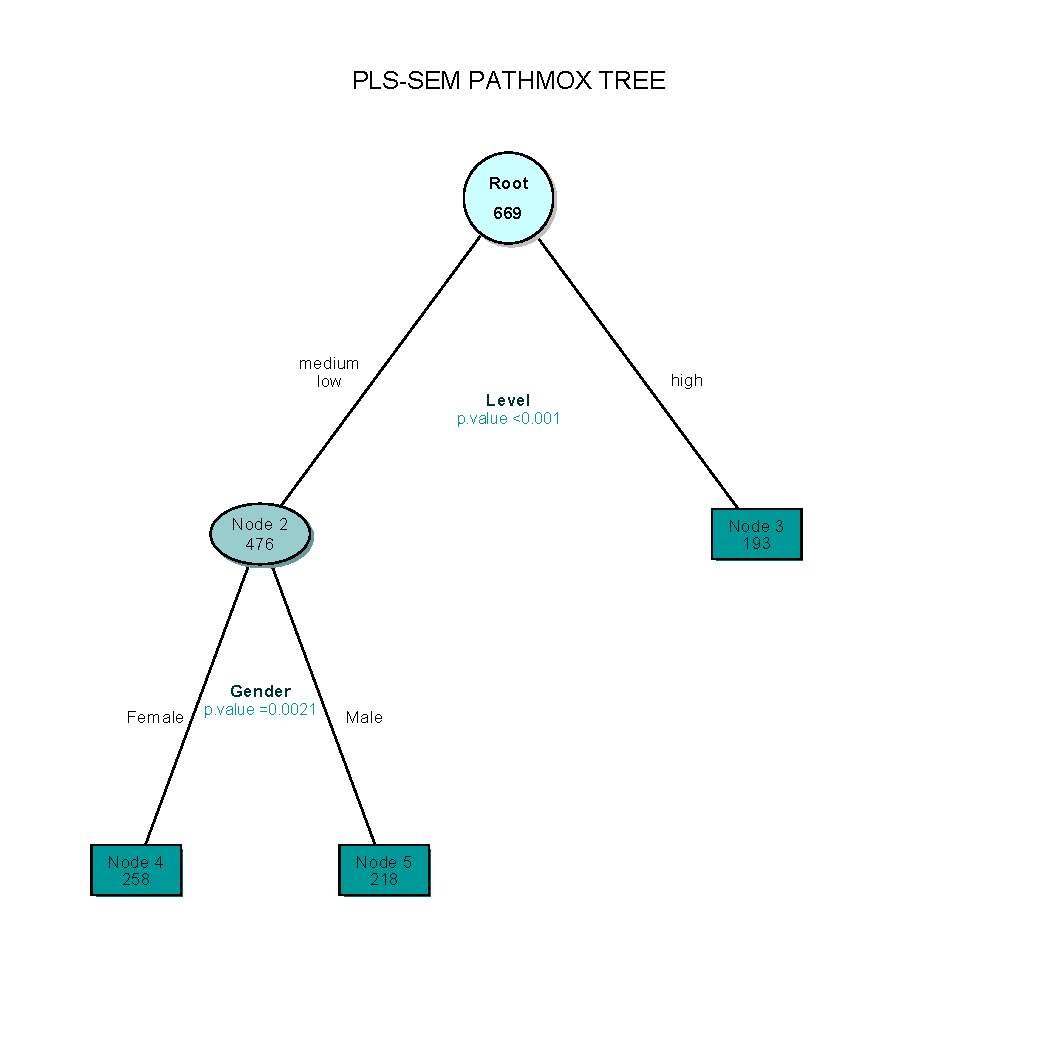
\includegraphics[width=0.6\textwidth]{Fig2_treeplot} &
    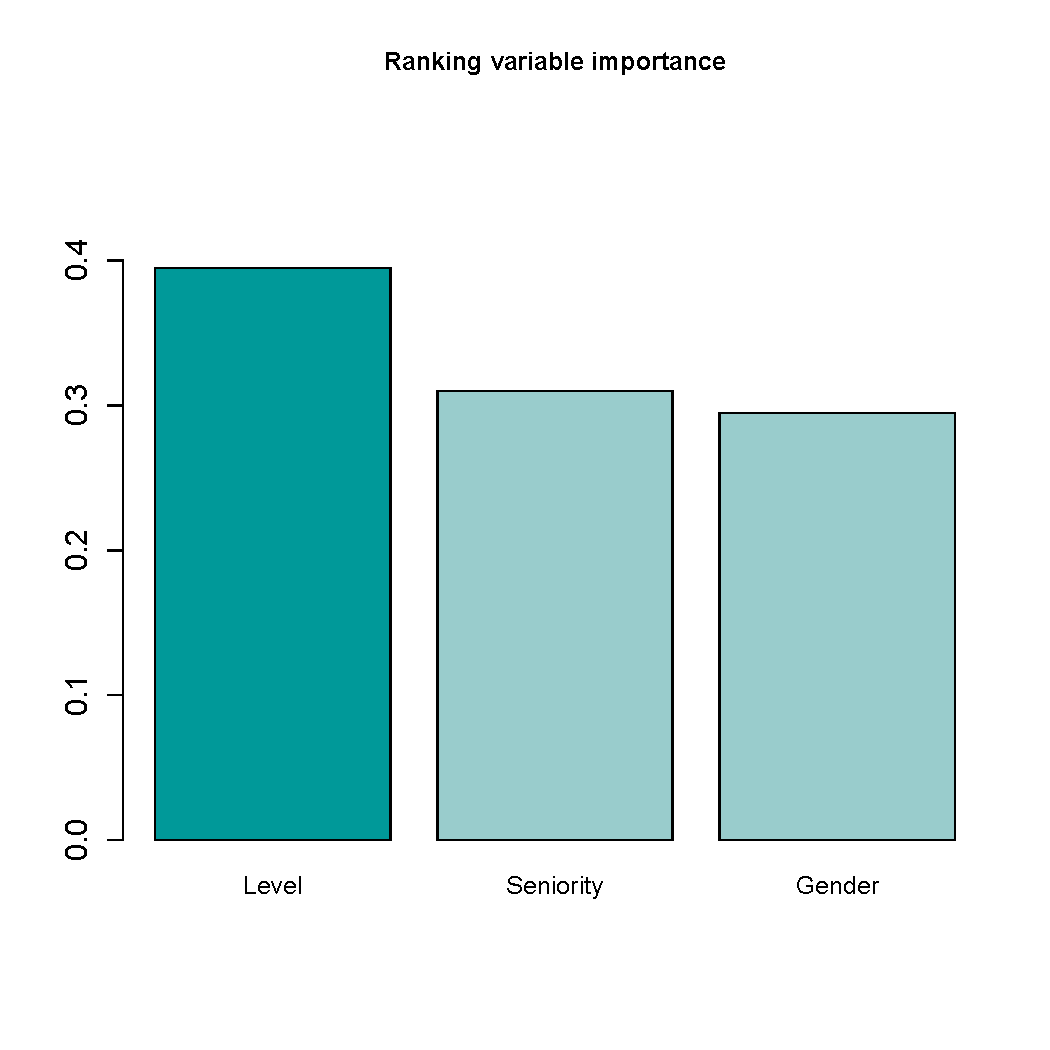
\includegraphics[width=0.4\textwidth]{FIg3_barimp}\\
    \multicolumn{2}{c}{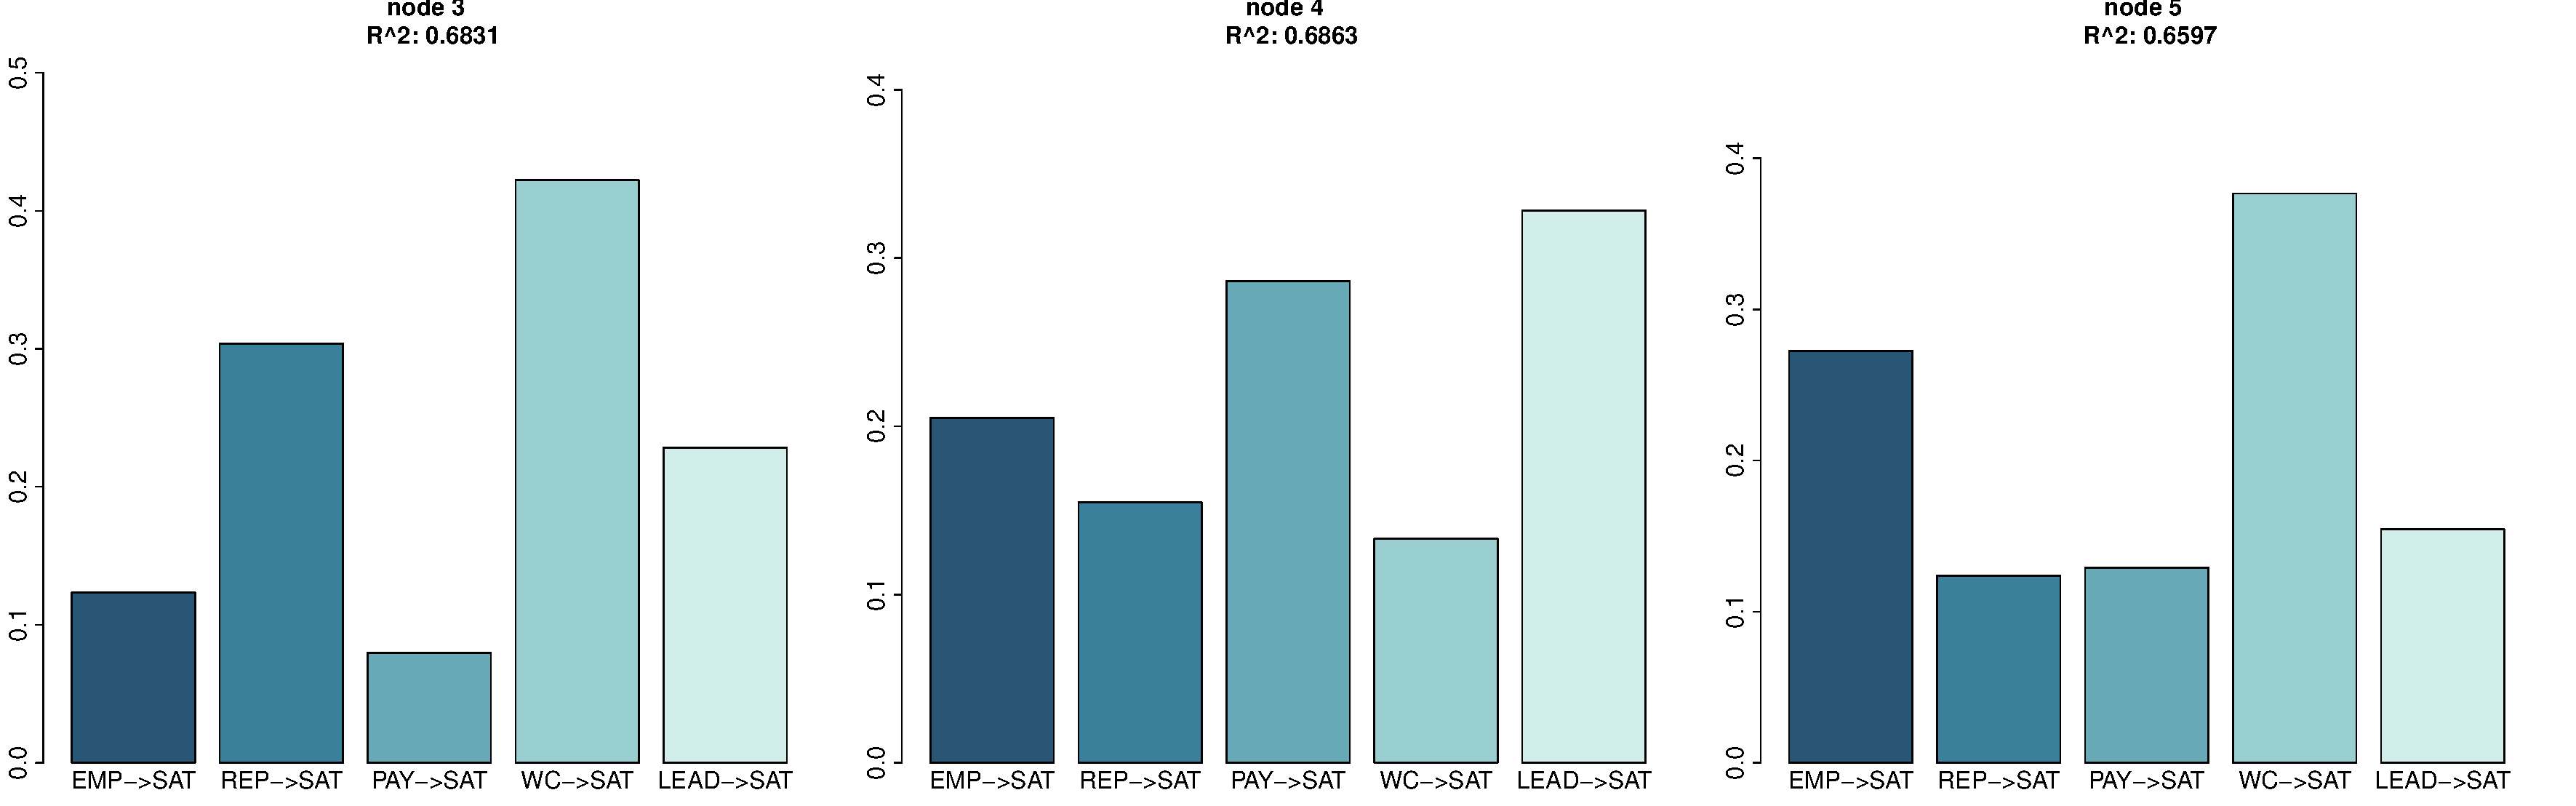
\includegraphics[width=1\textwidth]{Fig4_barcomp}}
\end{array}$
\caption[]{\label{vis} Plot types available in the genpathmox package: the treeplot (top left), the variable-importance ranking plot (top right), and  the barplot of the terminal nodes coefficients  (bottom)}
\end{figure*}


\subsection{Terminal node outputs}

Specific terminal nodes can be analyzed using the  \pkg{cSEM} package function  \code{csem()}. By default the  \code{csem()} function needs two parameters: the datasets that include all indicators (\code{.data}), and the PLS-SEM model relationships (\code{.model}).  As we are interested in the results of the terminal nodes, we pass the \code{hybrid} list in the "\code{plstree}" object to the \code{.data} parameter, and use the same formula object defined for the  \code{pls.pathmox()} function. Below we reproduce the code, but not the output, as not directly related with the \pkg{genpathmox} package. 

\begin{example}

# load cSEM package
library(cSEM)

# identify terminal nodes
terminal_nodes_data = climate.pathmox$hybrid

# terminal nodes results 
terminal_nodes_results = csem(.data = terminal_nodes_data, 
						.model = climate_model)
\end{example}

\subsection{Hybrid multigroup approach \citep{Lamberti21}: invariance and multigroup analysis}

For the invariance and the multigroup comparison of the terminal nodes identified by pathmox, we pass the object generated by the \code{csem()} function to the \code{testMICOM()} and  \code{testMGD()} functions. Note that, for the multigroup comparison, we need to indicate which coefficients to compare by fixing the parameter 
 \code{.parameters\_to\_compare}. We generate the work climate model,  but this time only indicating the causal relationship between the LVs. Finally, we indicate which statistical test to use for comparison using the \code{.approach\_mgd} parameter (for our example, the permutation test, \code{.approach\_mgd = }"\code{Chin}"). Below we reproduce the code to show how \pkg{genpathmox} interfaces with \pkg{cSEM}, omitting the results as there are not directly produced by the \pkg{genpathmox} package.
 
 \begin{example}
# MICOM procedure
climateMICOM = testMICOM(terminal_nodes_results)

# define the relationship between LVs
climateMICOM = testMICOM(terminal_nodes_results)

climate_innermodel = "
	# Structural model
	SAT ~ EMP + REP + PAY + WC + LEAD
	LOY ~   SAT
	"
# multigroup analysis
climateMGA = testMGD(terminal_nodes_results, 
					.parameters_to_compare = climate_innermodel,
                     		   .approach_mgd = "Chin")

\end{example}

\section{Summary}

The \pkg{genpathmox} \emph{R} package handles observed heterogeneity in PLS-SEM models when the number of CVs is high and we do not know what the most significant groupings could be. Development of \pkg{genpathmox} reflects the statistical framework described in \citet{Lamberti21}, and  \citet{Lamberti17, Lamberti16}, and the package has several functions that enable estimation and visualization of tree partitions.  By using \pkg{genpathmox}, users can quickly explore the effects of heterogeneity on their PLS-SEM models and identify groups that may contribute to significant differences.




\bibliography{Lamberti.bib}

\address{Giuseppe Lamberti,\\
  Department of Business,\\
  Universitat Autonoma de Barcelona UAB,\\
  Spain.\\
  http://orcid.org/0000-0002-8666-796X\\
  \email{giuseppe.lamberti@uab.cat}}


